\subsubsection*{Informazioni sul package}
\begin{figure}[h]
	\centering
	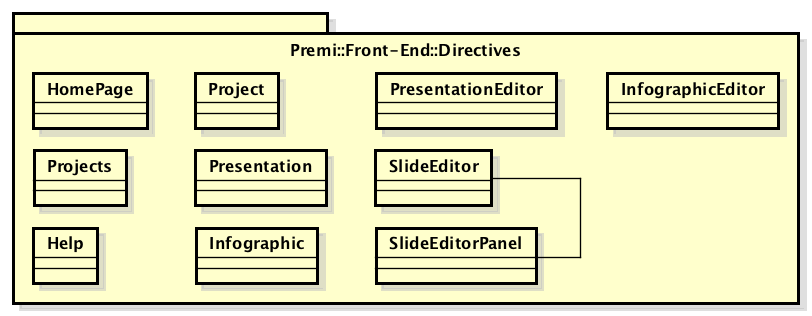
\includegraphics[width=0.9\linewidth]{img/front-end_directives}
	\caption[Premi::Front-End::Directives]{Premi::Front-End::Directives}
\end{figure}
\begin{itemize}
	\item \textbf{Descrizione}: Il package contiene gli elementi per creare le direttive del \gls{front-end}, ovvero per creare gli oggetti che consentono di richiamare le view e di collegarle ai rispettivi controller.
	\item \textbf{Interazione con altri package}:
	\begin{itemize}
		\item Vi è un'interazione con il package Premi::Front-End::Model poiché in esso vengono depositati e prelevati i dati necessari alle view richieste;
		\item Vi è un'interazione con il package Premi::Front-End::Services responsabile del recupero e salvataggio delle informazioni e dell'invocazione di precise procedure dall'esterno mediante chiamate REST.
	\end{itemize}
\end{itemize}

\subsubsection*{Classi contenute}
\begin{itemize}
	\item Premi::Front-End::Directives::HomePage:
	\begin{itemize}
		\item \textbf{Descrizione}: classe per la gestione della componente grafica della home page e del rispettivo controller, permettendo di raggiungere i link per la ricerca di un progetto, il login al sito e la registrazione ad esso.
	\end{itemize}

    \item Premi::Front-End::Directives::Projects:
	\begin{itemize}
		\item \textbf{Descrizione}: classe per la gestione della componente grafica della pagina relativa ai progetti creati da un utente e del rispettivo controller. Permette di aprire il progetto desiderato;
		\item \textbf{Relazioni con altre classi}:
		\begin{itemize}
			\item Premi::Front-End::Controllers::ProjectsController;
			\item Premi::Front-End::Views::ProjectsView.
		\end{itemize}
	\end{itemize}

    \item Premi::Front-End::Directives::Help:
	\begin{itemize}
		\item \textbf{Descrizione}: classe per la gestione della componente grafica dell'help al sito e del rispettivo controller, permettendo di visualizzare la guida all'utilizzo dell'applicazione.
	\end{itemize}

    \item Premi::Front-End::Directives::Project:
	\begin{itemize}
		\item \textbf{Descrizione}: classe per la gestione della componente grafica della pagina relativa al progetto aperto e del rispettivo controller;
		\item \textbf{Relazioni con altre classi}:
		\begin{itemize}
			\item Premi::Front-End::Controllers::ProjectController;
			\item Premi::Front-End::Views::ProjectView.
		\end{itemize}
	\end{itemize}

    \item Premi::Front-End::Directives::Presentation:
	\begin{itemize}
		\item \textbf{Descrizione}: classe per la gestione della visualizzazione della presentazione una volta che è stata creata e del rispettivo controller. Permette poi di interagire con il sistema fornendo tutti i comandi necessari allo scopo;
		\item \textbf{Relazioni con altre classi}:
		\begin{itemize}
			\item Premi::Front-End::Controllers::PresentationController;
			\item Premi::Front-End::Views::PresentationView.
		\end{itemize}
	\end{itemize}

    \item Premi::Front-End::Directives::PresentationEditor:
	\begin{itemize}
		\item \textbf{Descrizione}: classe per la gestione della componente grafica relativa alla modifica di una presentazione e del rispettivo controller. Richiama al suo interno la direttiva per la modifica della singola slide;
		\item \textbf{Relazioni con altre classi}:
		\begin{itemize}
			\item Premi::Front-End::Controllers::PresentationEditorController;
			\item Premi::Front-End::Views::PresentationEditorView.
		\end{itemize}
	\end{itemize}

    \item Premi::Front-End::Directives::SlideEditor:
	\begin{itemize}
		\item \textbf{Descrizione}: classe per la gestione della componente grafica relativa alla modifica di una slide e del rispettivo controller;
		\item \textbf{Relazioni con altre classi}:
		\begin{itemize}
			\item Premi::Front-End::Controllers::SlideEditorController;
			\item Premi::Front-End::Views::SlideEditorView.
		\end{itemize}
	\end{itemize}

    \item Premi::Front-End::Directives::SlideEditorPanel:
	\begin{itemize}
		\item \textbf{Descrizione}: classe per la gestione della componente grafica relativa al pannello di modifica di un componente durante la modifica di una slide e del rispettivo controller. Dà accesso alle proprietà di ogni componente;
		\item \textbf{Relazioni con altre classi}:
		\begin{itemize}
			\item Premi::Front-End::Controllers::SlideEditorController;
			\item Premi::Front-End::Views::SlideEditorPanelView.
		\end{itemize}
	\end{itemize}

    \item Premi::Front-End::Directives::Infographic:
	\begin{itemize}
		\item \textbf{Descrizione}: classe per la gestione della componente grafica relativa alla visualizzazione di un'\gls{infografica} e del rispettivo controller. Permette di accedere al tool di modifica dell'\gls{infografica};
		\item \textbf{Relazioni con altre classi}:
		\begin{itemize}
			\item Premi::Front-End::Controllers::InfographicEditorController;
			\item Premi::Front-End::Views::InfographicView.
		\end{itemize}
	\end{itemize}

    \item Premi::Front-End::Directives::InfographicEditor:
	\begin{itemize}
		\item \textbf{Descrizione}: classe per la gestione della componente grafica relativa alla creazione e modifica di un'\gls{infografica} e del rispettivo controller;
		\item \textbf{Relazioni con altre classi}:
		\begin{itemize}
			\item Premi::Front-End::Controllers::InfographicEditorController;
			\item Premi::Front-End::Views::InfographicView.
		\end{itemize}
	\end{itemize}

\end{itemize}
